\input{permve-ntnu-latex-assignment.tex}

\usepackage{float}
\usepackage[htt]{hyphenat}
\usepackage{tabularx}

\newacro{EA}{Evolutionary Algorithm}
\newacro{LOLZ}{Leading-One Leading-Zero}

\title{
\normalfont \normalsize
\textsc{Norwegian University of Science and Technology\\IT3708 -- Subsymbolic Methods in AI}
\horrule{0.5pt} \\[0.4cm]
\huge Project 2:\\ Programming an \acf{EA}\\
\horrule{2pt} \\[0.5cm]
}

\author{Per Magnus Veierland\\permve@stud.ntnu.no}

\date{\normalsize\today}

\pgfplotsset{compat=1.5}

\pgfplotsset{
every axis/.append style={
scale only axis,
width=0.40\textwidth,height=0.3\textwidth,
},
/tikz/every picture/.append style={
trim axis left,
trim axis right,
baseline
}
}

\begin{document}

\fancyfoot[C]{}
\maketitle

\newpage
\fancyfoot[C]{\thepage~of~\pageref{LastPage}} % Page numbering for right footer
\setcounter{page}{1}

\section*{Program implementation}

The \ac{EA} framework for this assignment is written in \textsc{C++14} and consists of a \texttt{individual} class which holds the genotype representation, the optional phenotype representation, and the fitness score; representation classes, e.g. \texttt{dynamic\_bit\_vector} with a matched function to spawn an instance of the representation, e.g. \texttt{dynamic\_bit\_vector\_creator}. Further it has classes to handle adult selection; \texttt{full\_generational\_replacement}, \texttt{generational\_mixing}, etc. Truthfully, the adult selection classes are best described as ``generational replacement policy'' classes, since they decide how to apply a reproduction function and develop the resulting children until the next generation has been built according to the policy. Further there are parent selection classes, \texttt{fitness\_proportionate}, \texttt{rank}, etc. which are used to select a single parent from a population. Reproduction classes, for which there currently is only \texttt{sexual}, are used to produce a set of children according to the reproduction policy, given a population and a parent selection policy. The reproduction class is responsible for invoking the selection of two parents, and applying crossover and mutation operators to form the resulting children. A \texttt{system} class is used to contain the parts and perform bookkeeping, but all evolution logic is handled by the parts.

As an example, the following shows how the \textsc{One-Max} fitness function is written as a lambda:

\begin{center}
{\footnotesize\texttt{
[] (const auto\& genotype)\\
\{ return static\_cast<double>(genotype.count()) / static\_cast<double>(genotype.size()); \}}}
\end{center}

\section*{\textsc{One-Max}}

When analyzing the \textsc{One-Max} problem with full-generational replacement, there will always be a chance of regression where fit individuals are replaced by less fit individuals. To consistently find a solution to the 40-bit \textsc{One-Max} problem in less than 100 generations with full-generational replacement, proportional fitness parent selection, 1~crossover point, a crossover rate of 1.0, and a mutation rate of 0.001, a population of 300~individuals was found to be appropriate. Across 100~runs, a population size of 300~individuals was found to consistently yield a valid solution. The mentioned parameter values are used as defaults in all comparisons.

The comparison of mutation rates (Figure~\ref{fig:onemax_mut}) shows that a mutation rate of 0.001 clearly outperforms 0.01 and 0.005 for this problem. It appears that a mutation rate between 0.0001 and 0.0005 results in the best performance for this problem.

Comparisons of crossover rates (Figure~\ref{fig:onemax_cross}) did not show any clearly superior options, and that crossover rates between 0.8 and 1.0 seems to result in the best performance.

Parent selection methods are compared in Figure~\ref{fig:onemax_parens}. Rank selection clearly outperforms proportionate fitness selection, and sigma selection clearly outperforms rank selection. It can further be observed that tournament selection is the best parent selection mechanism for the problem, and that smaller tournament groups perform better than larger tournament groups.

\newcommand{\displayplots}[2]{
    \addplot[#2, mark=none] table[x index=0,y index=2,col sep=space] {../data/#1-run-1.txt};
    \addplot[#2, mark=none] table[x index=0,y index=2,col sep=space] {../data/#1-run-2.txt};
    \addplot[#2, mark=none] table[x index=0,y index=2,col sep=space] {../data/#1-run-3.txt};
    \addplot[#2, mark=none] table[x index=0,y index=2,col sep=space] {../data/#1-run-4.txt};
    \addplot[#2, mark=none] table[x index=0,y index=2,col sep=space] {../data/#1-run-5.txt};
    \addplot[#2, mark=none, densely dotted] table[x index=0,y index=1,col sep=space] {../data/#1-run-1.txt};
    \addplot[#2, mark=none, densely dotted] table[x index=0,y index=1,col sep=space] {../data/#1-run-2.txt};
    \addplot[#2, mark=none, densely dotted] table[x index=0,y index=1,col sep=space] {../data/#1-run-3.txt};
    \addplot[#2, mark=none, densely dotted] table[x index=0,y index=1,col sep=space] {../data/#1-run-4.txt};
    \addplot[#2, mark=none, densely dotted] table[x index=0,y index=1,col sep=space] {../data/#1-run-5.txt};
}

\begin{figure}
\centering
\begin{tabularx}{\textwidth}{XcXc}
~ &
\begin{tikzpicture}
\begin{axis}[xlabel={Generation},ylabel={Mean population fitness}, legend pos=south east]
\addlegendentry{M=0.01}
\addlegendentry{M=0.005}
\addlegendentry{M=0.001}
\addlegendimage{no markers,red}
\addlegendimage{no markers,green}
\addlegendimage{no markers,blue}
\displayplots{onemax-adult-proportionate-crossover-1.0-mutation-0.01-population-300-problem-40-generations-100}{red}
\displayplots{onemax-adult-proportionate-crossover-1.0-mutation-0.005-population-300-problem-40-generations-100}{green}
\displayplots{onemax-adult-proportionate-crossover-1.0-mutation-0.001-population-300-problem-40-generations-100}{blue}
\end{axis}
\end{tikzpicture}
& ~ &
\begin{tikzpicture}
\begin{axis}[xlabel={Generation},ylabel={Mean population fitness}, legend pos=south east]
\addlegendentry{M=0.001}
\addlegendentry{M=0.0005}
\addlegendentry{M=0.0001}
\addlegendimage{no markers,blue}
\addlegendimage{no markers,yellow}
\addlegendimage{no markers,black}
\displayplots{onemax-adult-proportionate-crossover-1.0-mutation-0.001-population-300-problem-40-generations-100}{blue}
\displayplots{onemax-adult-proportionate-crossover-1.0-mutation-0.0005-population-300-problem-40-generations-100}{yellow}
\displayplots{onemax-adult-proportionate-crossover-1.0-mutation-0.0001-population-300-problem-40-generations-100}{black}
\end{axis}
\end{tikzpicture}
\\
\end{tabularx}
\caption{\textsc{One-Max} mutation rate comparison}
\label{fig:onemax_mut}
\end{figure}

\begin{figure}
\centering
\begin{tabularx}{\textwidth}{XcXc}
~ &
\begin{tikzpicture}
\begin{axis}[xlabel={Generation},ylabel={Mean population fitness}, legend pos=south east]
\addlegendentry{C=1.0}
\addlegendentry{C=0.8}
\addlegendentry{C=0.6}
\addlegendimage{no markers,red}
\addlegendimage{no markers,green}
\addlegendimage{no markers,blue}
\displayplots{onemax-adult-proportionate-crossover-1.0-mutation-0.0001-population-150-problem-40-generations-100}{red}
\displayplots{onemax-adult-proportionate-crossover-0.8-mutation-0.0001-population-150-problem-40-generations-100}{green}
\displayplots{onemax-adult-proportionate-crossover-0.6-mutation-0.0001-population-150-problem-40-generations-100}{blue}
\end{axis}
\end{tikzpicture}
& ~ &
\begin{tikzpicture}
\begin{axis}[xlabel={Generation},ylabel={Mean population fitness}, legend pos=south east]
\addlegendentry{C=0.98}
\addlegendentry{C=0.95}
\addlegendentry{C=0.92}
\addlegendimage{no markers,purple}
\addlegendimage{no markers,yellow}
\addlegendimage{no markers,black}
\displayplots{onemax-adult-proportionate-crossover-0.98-mutation-0.0001-population-150-problem-40-generations-100}{blue}
\displayplots{onemax-adult-proportionate-crossover-0.95-mutation-0.0001-population-150-problem-40-generations-100}{yellow}
\displayplots{onemax-adult-proportionate-crossover-0.92-mutation-0.0001-population-150-problem-40-generations-100}{black}
\end{axis}
\end{tikzpicture}
\\
\end{tabularx}
\caption{\textsc{One-Max} crossover rate comparison}
\label{fig:onemax_cross}
\end{figure}

\begin{figure}
\centering
\begin{tabularx}{\textwidth}{XcXc}
~ &
\begin{tikzpicture}
\begin{axis}[xlabel={Generation},ylabel={Mean population fitness}, legend pos=south east]
\addlegendentry{Proportionate}
\addlegendentry{Rank}
\addlegendentry{Sigma}
\addlegendimage{no markers,red}
\addlegendimage{no markers,green}
\addlegendimage{no markers,blue}
\displayplots{onemax-adult-proportionate-crossover-1.0-mutation-0.0001-population-300-problem-40-generations-100}{red}
\displayplots{onemax-adult-rank-crossover-1.0-mutation-0.0001-population-300-problem-40-generations-100}{green}
\displayplots{onemax-adult-sigma-crossover-1.0-mutation-0.0001-population-300-problem-40-generations-100}{blue}
\end{axis}
\end{tikzpicture}
& ~ &
\begin{tikzpicture}
\begin{axis}[xlabel={Generation},ylabel={Mean population fitness}, legend pos=south east]
\addlegendentry{Tournament (10)}
\addlegendentry{Tournament (25)}
\addlegendentry{Tournament (50)}
\addlegendimage{no markers,purple}
\addlegendimage{no markers,yellow}
\addlegendimage{no markers,black}
\displayplots{onemax-adult-tournament-group-10-crossover-1.0-mutation-0.0001-population-300-problem-40-generations-100}{purple}
\displayplots{onemax-adult-tournament-group-25-crossover-1.0-mutation-0.0001-population-300-problem-40-generations-100}{yellow}
\displayplots{onemax-adult-tournament-group-50-crossover-1.0-mutation-0.0001-population-300-problem-40-generations-100}{black}
\end{axis}
\end{tikzpicture}
\\
\end{tabularx}
\caption{\textsc{One-Max} parent selection comparison}
\label{fig:onemax_parent}
\end{figure}

\section*{\acf{LOLZ}}

\begin{figure}
\centering
\begin{tabularx}{\textwidth}{XcX}
~ &
\begin{tikzpicture}
\begin{axis}[xlabel={Generation},ylabel={Best population fitness}, legend pos=south east, cycle list name=color list, mark=none]
\addplot[black, mark=none] table[x index=0,y index=1,col sep=space] {../data/lolz-adult-tournament-10-crossover-1.0-mutation-0.0001-population-300-L-40-Z-21-generations-500-run-1.txt};
\addplot[black, mark=none] table[x index=0,y index=1,col sep=space] {../data/lolz-adult-tournament-10-crossover-1.0-mutation-0.0001-population-300-L-40-Z-21-generations-500-run-2.txt};
\addplot[black, mark=none] table[x index=0,y index=1,col sep=space] {../data/lolz-adult-tournament-10-crossover-1.0-mutation-0.0001-population-300-L-40-Z-21-generations-500-run-3.txt};
\addplot[black, mark=none] table[x index=0,y index=1,col sep=space] {../data/lolz-adult-tournament-10-crossover-1.0-mutation-0.0001-population-300-L-40-Z-21-generations-500-run-4.txt};
\addplot[black, mark=none] table[x index=0,y index=1,col sep=space] {../data/lolz-adult-tournament-10-crossover-1.0-mutation-0.0001-population-300-L-40-Z-21-generations-500-run-5.txt};
\addplot[black, mark=none] table[x index=0,y index=1,col sep=space] {../data/lolz-adult-tournament-10-crossover-1.0-mutation-0.0001-population-300-L-40-Z-21-generations-500-run-6.txt};
\addplot[black, mark=none] table[x index=0,y index=1,col sep=space] {../data/lolz-adult-tournament-10-crossover-1.0-mutation-0.0001-population-300-L-40-Z-21-generations-500-run-7.txt};
\addplot[black, mark=none] table[x index=0,y index=1,col sep=space] {../data/lolz-adult-tournament-10-crossover-1.0-mutation-0.0001-population-300-L-40-Z-21-generations-500-run-8.txt};
\end{axis}
\end{tikzpicture}
& ~ \\
\end{tabularx}
\caption{Comparison of 8 runs for the \textsc{LOLZ} problem with full generational replacement, tournament parent selection (10), one-point crossover and mutation rate 0.0001, population 300.}
\label{fig:lolz_runs}
\end{figure}

\section*{Surprising Sequences}

Figure~\ref{fig:surprising_genotype} shows the integer vector genotype used to represent individuals for the surprising sequence problem. In addition to representing an individual as an integer vector, the symbol set size $S$ is also stored. This value is used when mutating the individual, such that mutating any position in the vector involves setting its value to a random member of the symbol set.

As no obvious advantage was seen in using a separate phenotype representation, individuals use the same representation for its genotype and effective phenotype.

\begin{figure}[H]
\centering
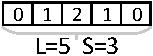
\includegraphics[scale=1.0]{images/surprising_genotype}
\caption{Surprising sequences integer vector genotype}
\label{fig:surprising_genotype}
\end{figure}

The fitness function for both local and global surprising sequences is based on the function \texttt{collisions}, which takes a sequence parameter, the symbol set size ($S$), and the pair distance to test for; $d$. The function counts collisions by iterating over each position, $i$, in the sequence. If the pair consisting of the symbol at position $i$ and the symbol at position $i+d+1$ has not been encountered, it is marked as seen in a lookup table. However, if the pair has already been seen as part of the \texttt{collisions} function invocation, it is recorded in the sum of collisions which the function ends up returning.

The local fitness function (Equation~\ref{eq:ss_local}) is based on a single call to the \texttt{collisions} function for the case $d=0$, while the global fitness function (Equation~\ref{eq:ss_global}) invokes the \texttt{collisions} function once for each $d$ in the range $[0, L-3]$. Each fitness function will result in a fitness of 1 in the case of no collisions, and scoring any addition in the number of collisions with a worse fitness.

\begin{equation}
\label{eq:ss_local}
\textit{fitness}_\textit{local} = \frac{1}{1 + \texttt{collisions}(\textit{sequence}, S, 0)}
\end{equation}

\begin{equation}
\label{eq:ss_global}
\textit{fitness}_\textit{global} = \frac{1}{1 + \sum_{d=0}^{L - 3} \texttt{collisions}(\textit{sequence}, S, d)}
\end{equation}

\begin{table}
{\tiny
\begin{tabularx}{\textwidth}{cccX}
\toprule
$S$ & $L$ & Gen. & Sequence \\
\midrule
3   & 10  & 0   & 2, 0, 0, 2, 2, 1, 0, 1, 1, 2 \\
5   & 26  & 39  & 4, 4, 0, 2, 1, 3, 4, 3, 3, 1, 2, 3, 2, 4, 1, 1, 0, 1, 4, 2, 2, 0, 3, 0, 0, 4 \\
10  & 100 & 2825 & 2, 0, 8, 9, 1, 5, 5, 0, 0, 1, 4, 3, 6, 8, 2, 8, 8, 7, 5, 9, 6, 2, 9, 7, 3, 2, 5, 3, 5, 6, 9, 8, 1, 8, 5, 1, 9, 3, 1, 7, 6, 6, 4, 0, 2, 2, 3, 9, 0, 5, 8, 0, 7, 1, 6, 3, 3, 8, 4, 7, 9, 4, 5, 4, 4, 2, 6, 0, 3, 4, 6, 7, 8, 6, 5, 2, 1, 0, 9, 2, 7, 4, 1, 2, 4, 8, 3, 0, 4, 9, 5, 7, 7, 0, 6, 1, 1, 3, 7, 2 \\
15  & 215 & 2435 & 0, 10, 10, 14, 11, 13, 6, 8, 8, 1, 12, 1, 2, 12, 2, 13, 0, 7, 9, 11, 1, 14, 7, 2, 9, 4, 2, 0, 1, 0, 3, 13, 3, 10, 5, 0, 11, 4, 14, 13, 9, 13, 14, 8, 9, 0, 14, 2, 6, 10, 12, 14, 6, 9, 9, 12, 3, 0, 2, 7, 3, 14, 12, 5, 5, 9, 6, 0, 5, 3, 6, 14, 3, 11, 12, 13, 1, 3, 1, 13, 12, 12, 0, 12, 11, 11, 7, 14, 4, 1, 9, 8, 6, 2, 4, 12, 8, 2, 14, 5, 12, 6, 7, 4, 4, 0, 9, 3, 4, 11, 0, 0, 6, 4, 8, 4, 7, 10, 11, 3, 3, 5, 7, 6, 1, 5, 8, 10, 3, 8, 7, 5, 2, 11, 14, 9, 7, 1, 8, 12, 9, 14, 0, 8, 0, 4, 10, 2, 8, 11, 9, 5, 4, 13, 7, 7, 13, 13, 8, 3, 2, 10, 7, 12, 10, 4, 9, 10, 0, 13, 10, 6, 3, 9, 2, 1, 6, 11, 5, 14, 1, 1, 10, 8, 5, 13, 2, 2, 3, 7, 11, 6, 12, 7, 8, 14, 14, 10, 1, 4, 6, 5, 6, 6, 13, 11, 2, 5, 10, 13, 5, 1, 11, 8, 13 \\
20  & 380 & 2923 & 7, 6, 14, 3, 7, 8, 13, 3, 9, 12, 16, 0, 13, 19, 19, 7, 16, 2, 9, 9, 19, 16, 10, 10, 7, 15, 12, 6, 8, 18, 18, 9, 14, 12, 19, 12, 18, 15, 14, 9, 6, 11, 17, 10, 11, 10, 1, 2, 11, 11, 5, 17, 9, 2, 12, 5, 8, 16, 19, 2, 17, 1, 14, 19, 3, 16, 12, 2, 8, 0, 6, 12, 12, 9, 1, 0, 11, 4, 0, 12, 10, 5, 13, 0, 19, 0, 15, 11, 16, 7, 1, 13, 7, 5, 15, 6, 17, 18, 3, 14, 2, 3, 10, 9, 7, 9, 3, 11, 3, 19, 1, 18, 5, 4, 13, 11, 19, 5, 5, 6, 2, 15, 5, 10, 12, 14, 7, 12, 17, 17, 5, 3, 3, 18, 2, 2, 13, 13, 9, 17, 12, 7, 18, 16, 8, 1, 3, 15, 19, 6, 0, 0, 17, 14, 16, 1, 8, 10, 8, 6, 9, 5, 1, 1, 16, 6, 3, 13, 16, 17, 8, 9, 18, 11, 12, 3, 12, 0, 16, 13, 1, 11, 15, 4, 17, 4, 14, 17, 6, 16, 3, 6, 1, 4, 2, 16, 14, 4, 8, 7, 14, 10, 18, 14, 11, 1, 6, 19, 11, 0, 1, 12, 11, 8, 17, 19, 9, 15, 2, 18, 6, 18, 0, 9, 16, 15, 7, 11, 7, 17, 13, 8, 5, 16, 16, 5, 18, 8, 12, 1, 7, 3, 8, 15, 8, 4, 16, 9, 0, 5, 11, 9, 11, 14, 6, 15, 0, 2, 10, 3, 2, 4, 19, 14, 15, 18, 10, 19, 4, 15, 1, 19, 15, 16, 18, 1, 9, 4, 6, 5, 19, 8, 2, 6, 6, 4, 12, 15, 9, 8, 14, 1, 15, 13, 12, 4, 1, 10, 6, 7, 19, 10, 13, 10, 0, 3, 4, 18, 7, 0, 18, 13, 5, 7, 4, 11, 18, 17, 0, 8, 11, 2, 0, 7, 7, 2, 14, 8, 8, 3, 1, 17, 16, 4, 4, 5, 2, 19, 13, 17, 11, 6, 13, 6, 10, 2, 1, 5, 9, 13, 15, 17, 15, 3, 17, 3, 0, 10, 17, 2, 5, 14, 5, 0, 14, 18, 19, 18, 4, 7, 13, 18, 12, 13, 14, 14, 0, 4, 3, 5 \\
\bottomrule
\end{tabularx}
}
\caption{Local surprising sequences (population: 200)}
\label{table:local_surprising}
\end{table}

\begin{table}
{\tiny
\begin{tabularx}{\textwidth}{cccX}
\toprule
$S$ & $L$ & Gen. & Sequence \\
\midrule
3 & 7 & 0 & 1, 0, 2, 2, 1, 2, 0 \\
5 & 12 & 5 & 3, 4, 4, 0, 1, 2, 0, 3, 0, 2, 1, 4 \\
10 & 25 & 386 & 4, 7, 2, 6, 8, 0, 8, 4, 6, 9, 1, 0, 3, 1, 5, 8, 2, 2, 5, 7, 4, 9, 3, 8, 6 \\
15 & 37 & 6042 & 2, 5, 11, 8, 6, 10, 4, 7, 13, 4, 9, 12, 10, 1, 0, 9, 7, 14, 3, 3, 13, 12, 2, 9, 5, 4, 11, 1, 11, 0, 10, 6, 12, 8, 14, 6, 7 \\
20 & 50 & 7135 & 1, 12, 15, 17, 14, 0, 3, 19, 6, 9, 11, 4, 1, 13, 2, 3, 5, 2, 19, 10, 17, 8, 7, 10, 14, 18, 13, 0, 8, 4, 5, 18, 0, 16, 13, 9, 6, 7, 6, 15, 5, 19, 11, 14, 12, 17, 3, 1, 1, 16 \\
\bottomrule
\end{tabularx}
}
\caption{Global surprising sequences (population: 200)}
\label{table:local_surprising}
\end{table}

\section*{Difficulty}

The \textsc{One-Max} problem was clearly the easiest problem, as there are no local maxima and only one correct solution for a given length. It is easy to write a good fitness function which reflects individual fitness well.

\textsc{LOLZ} is a harder problem than \textsc{One-Max} since it is designed to have a distinct local maxima, and because representations in the local maxima are exact opposites to the global maxima; it will be very hard to escape this local maxima for an \ac{EA}.

Surprising sequences is the hardest problem of the three due to the complexity and cost of the fitness evaluation, and due to the complexity of valid sequences.

\end{document}

